\chapter{Queries}
\label{chap:Queries}

A high performance database for OLAP workloads does not only rely on the data format, the compression, and the implementation. We find algorithms and optimization done in the queries to be important for good performance.
\newpage

\section{General considerations}
\label{sec:General considerations}
We find one of the most important technique for good query performance to operate directly on compressed data. This is especially when using dictionary compression, such that equal predicates can be performed by a simple integer operation \cite{Abadi2008-dd}. Systems querying direcly on compressed data are \cstore, \ibm, \mssql, \blink, \saph. When dictionary compression is used, keys from the inner join must be switched to keys of the outer join in the join process \cite{Raman2013-em}.

We see that some systems also make a distinction between measure and dimension attributes \cite{Kamkolkar2015-iq, Johnson2008-cp}. Knowing this about a column might aid in data placement, and we believe it can be used for making decisions about index generation.

\subsection{Query operators}
\label{sub:Query operators}
There are several operators that should be supported in SQL. \cstore supports Decompress, select, mask, Project, Sort, Aggregation operators, concat, permute, join, bitstring operators \cite{Stonebraker2005-qz}.

To simplify some of the queries, one may put restrictions to the SQL. Earlier versions of \mssql~did not support outer joins and group-by on scalar attributes \cite{Larson2013-mc}. This was justified as none of this was common for "datawarehouse scenarios".~


\section{Joining}
\label{sec:Joining}
Database joins are normally classified as either hash join or sort-merge join. Hash join is the most popular joining algorithm, especially in parallel \cite{Boncz2002-yj}. However, hash join can do ... and merge join can do ... \cite{DeWitt1992-ki}

\subsection{Hash join}
\label{sub:Hash join}
Hash join is performed by hashing the smaller (inner) relation first, then scan the outer relation where the hash table is probed. This is especially easy in a star or snowflake schema, where the dimensions are hashed, and the fact table is probed \cite{Barber2012-xt, Raman2013-em}

Another design goal is to keep the hash tables collision free \cite{Raman2013-em, Raman2008-gi}. Linear hashing is preferred over open-chain hashing due to better cache utilization \cite{Raman2008-gi}. Depending on the number of groups, perfect hashing should be used for lagre groups, and a method known as IDX for small.

There are ways of improving performance in the caching algorithms in terms of implementation details and cache awareness (Section ?). \monetdb~utilizies a radix cluster algorithms, where multiple passes are used to maximize cache locality \cite{Boncz2002-yj}. They find a performance improvement of 90\% using this technique. \mssql~implementation of the hash join still keeps good performance if some pages are allowed to be spilled to disk \cite{Larson2013-mc}. 

\begin{figure}
  \centering
  \begin{subfigure}{0.45\textwidth}
    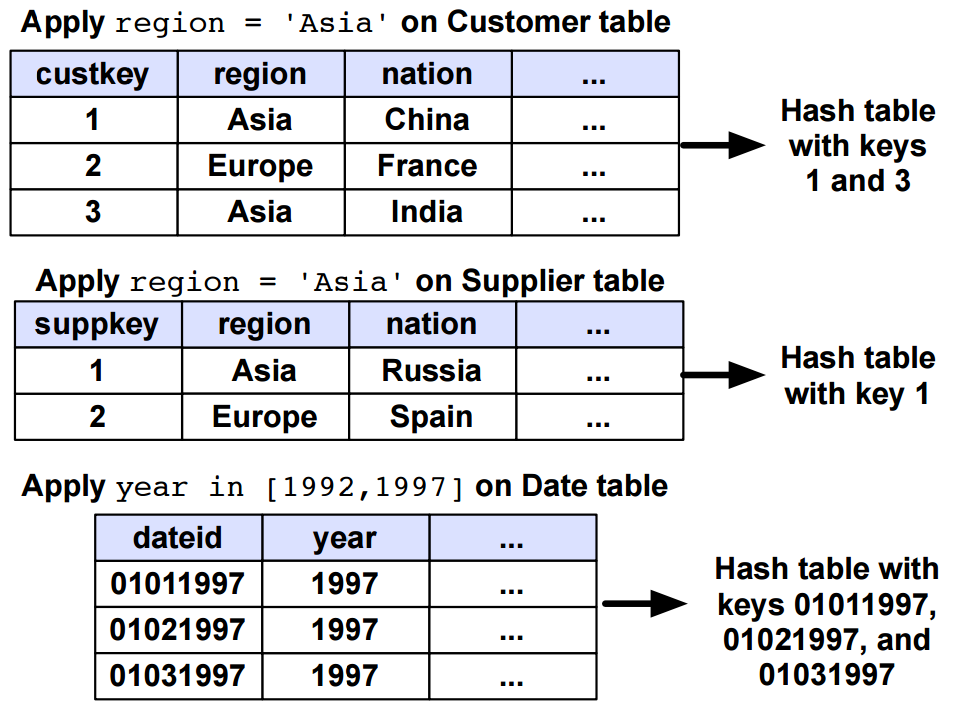
\includegraphics[width=\textwidth]{img/invisible-join-1.png}
    \caption{The first phase of the invisible join. Predicates are evaluated on every dimension table, and put into a hash map.}
    \label{fig:invisible-join-1} 
  \end{subfigure}
  \begin{subfigure}{0.45\textwidth}
    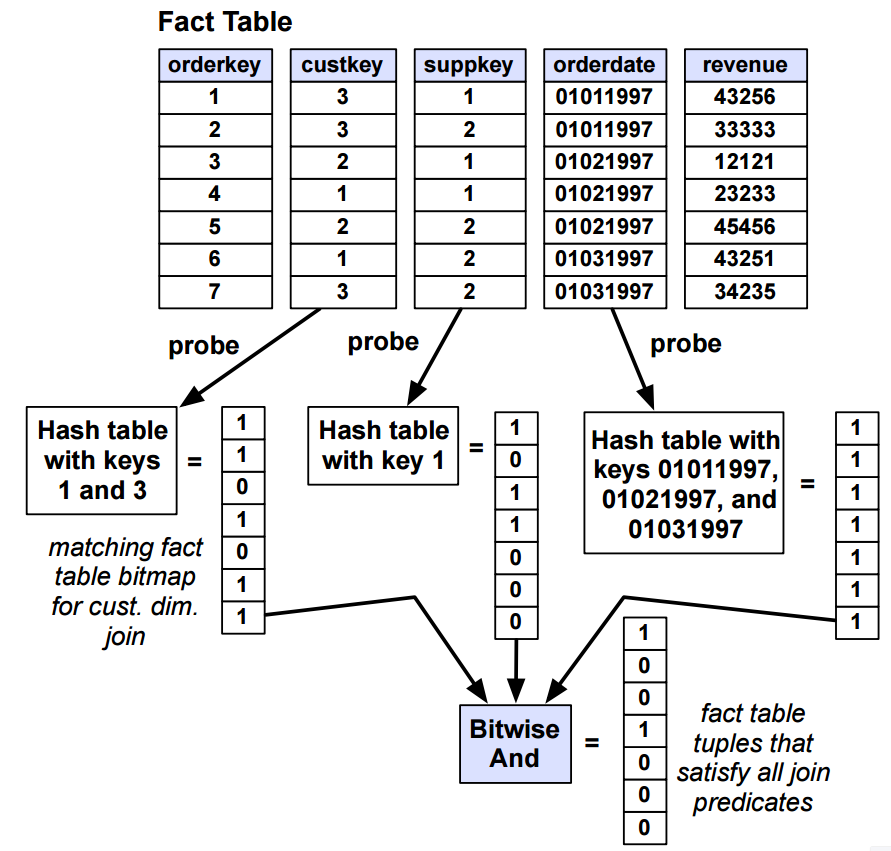
\includegraphics[width=\textwidth]{img/invisible-join-2.png}
    \caption{The second phase of the invisible join. Bitmaps are created per dimension table predicate, and bitwise \texttt{AND} is applied.}
    \label{fig:invisible-join-1} 
  \end{subfigure}
  \begin{subfigure}{0.45\textwidth}
    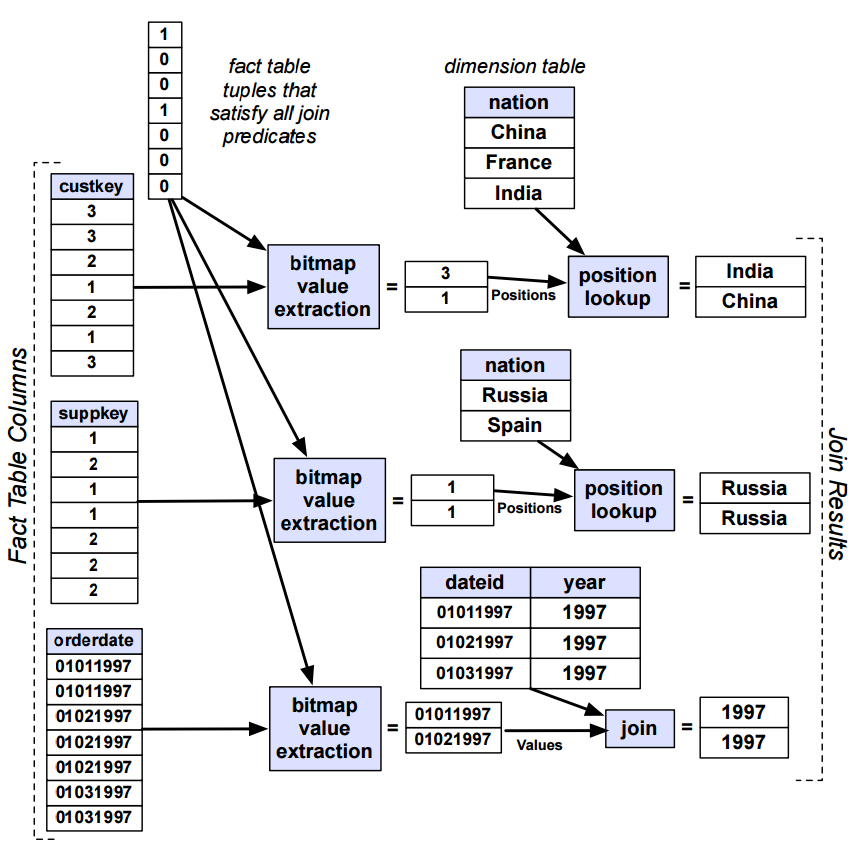
\includegraphics[width=\textwidth]{img/invisible-join-3.png}
    \caption{The third phase of the invisible join. The bitmap calculated in the previous step is uned to extract values from the fact table.}
    \label{fig:invisible-join-1} 
  \end{subfigure}
  \caption{The invisible join. Courtesy of \cite{Abadi2008-dd}.}
  \label{fig:invisible-join} 
\end{figure}
Another technique, introduced by Abadi \ea~in \term{invisible join} \cite{Abadi2008-dd}. Here, the set of tuples in the larger relation is reduced using selection predicates in one or many relation tables. For each predicate, a bitmap is produced. This is ANDed/ORed at the end of the query. Projected values are not fetched until the end. The whole join is depicted in Figure~\ref{fig:invisible-join}.

The most detailed research we find on hash join, is the work by Barber \ea~\cite{Barber2014-ey}. They explain how data independent ranmod access (DIRA) can build hash tables without contention, utilizing prefetching. Through the use of overflow hash tables, they reduce the amount of collisions and get 100\% occupancy. Hash tables are built in parallel.


\subsection{Bloom filter based joins}
\label{sub:Bloom filter based joins}
Although not directly compression, another way of reducing a bitmaps footprint and increasing query performance, is through the use of bloom filters \cite{Bloom1970-nr}. A bloom filter may return false positives, but never false negatives.The bloom filters can be used in common database operations, for instance joins \cite{x} \todo{Consider moving this somewhere else}. Several database systems report to use bloom filter based joins. Bloom filters, invented by Bloom in 1970, is a probabilistic structure and will only return false positives, not false negatives \cite{Bloom1970-nr}. This includes \oracle~\cite{Lahiri2015-mz}, \ibm~\cite{Raman2013-em}. Barber \ea~explain how bloom filters can be applied to eliminate non-matching join outers before they enter the join.

\section{Predicate evaluation}
\label{sec:Predicate evaluation}
We see various techniques that improves the predicate evaluation.

It is common to use bitmaps in predicate evaluation \cite{Raman2008-gi, Raman2013-em}. In \blink, bitmaps are calculated and operations are performed directly on the bitmaps.

Predicates are also evaluated in a Single Input Multipe Data (SIMD) fashion, which is a technique described by Johnson \ea~\cite{Johnson2008-cp}. Extensive use of processor SIMD instructions is explained by Willhalm \ea~\cite{Willhalm2009-hu, Willhalm2013-ri}. Evaluating predicates in a SIMD like fashion is done in \blink~\cite{Raman2008-gi}.  This system reports a performance increase when three or more predicates are evaluated at the same time.

\section{Query optimization}
\label{sec:Query optimization}
Most of the database systems found in literature use some kind of query optimization. Query optimizers must seek to reduce the search space \cite{Boncz2002-yj, Stonebraker2005-qz}

\blink~makes query optimization much easier, since the only operation for evaluating predicates in a query is a scan operation \cite{Barber2012-xt}. In addition, joins and grouping is done in prespecified order. The core idea of this system is a generalized scan which performs scan, selection, groping, and aggregation \cite{Raman2008-gi}

It is important that the optimizer is "compression aware" \cite{Westmann200-mz}. The query optimizer must be aware that columns might be compressed, and that these compressed columns can be worked on directly without decompression \cite{Stonebraker2005-qz}

In addition, it is important to filter data as early as possible in the plan \cite{Lamb2012-kg}, and in join operation  most selective columns should be processed first \cite{Holloway2008-rr}. In a parallel settiong, the query optimizer should minimize the need for coordination \cite{Exasol2014-xh}.

Long in-lists can be turned into a precomputed hash table \cite{Raman2013-em}.

Queries must also use the available optimizations allowed by the design \cite{Barber2012-xt}. Metadata indexes (Section ?) can be used to skip blocks. Dictionaries can be checked, and partitions can be skipped entirely if the key is not present in the dictionary (Section ?). \texttt{LIKE} predicates can be turned into \texttt{IN} predicates based on the entries in the dictionary.

\section{Grouping and Aggregation}
\label{sec:Grouping and Aggregation}
Aggregation of results is also an important step of querying. It can be done at the same time as for the scan \cite{Leme2010-is}.

\ffigure{img/vector-group-by}{The \term{Vector Group By} technique used in \oracle. Courtesy of \cite{Oracle2015-fs}.}{fig:vector-group-by}
\oracle~uses a technique which they call \term{Vector Group By}, which is a compact multipdimensional array for storing aggregate results. The operation is depicted in Figure~\ref{fig:vector-group-by}.

\ibm~performs a local groping on local hash tables in parallel, and creates a linked list of overflow buckets \cite{Raman2013-em}. When they are full, they get published globally. In the second phase, each thread reserves a part of the hash table and merges the local hash tables to a global one.

Dictionary compresison can simplify the aggregation step, because the dicionary entries can be used directly for storing the aggregated results \cite{Lemke2010-is, Boncz2005-wj}. \blink~uses the dicitonary codes directly as group codes, which is a perfect hash \cite{Raman2008-gi}. If the query is grouped by multiple attributes, a minimal perfect hash is found. 

\section{Query structures}
\label{sec:Query structures}
\missingfigure{Selection vector illustration from \cite{Boncz2005-wj}}
If the queries work on vectors at a time (vectorized execution, section X), the auxiliary structure in \monetx~is a selection vector \cite{Boncz2005-wj}.



